\documentclass[conference]{IEEEtran}
\IEEEoverridecommandlockouts
\usepackage{cite}
\usepackage{amsmath,amssymb}
\usepackage{graphicx}
\usepackage{booktabs}
\usepackage[table]{xcolor}
\usepackage[bookmarks=false]{hyperref}
\hypersetup{hidelinks}
\hbadness=10000
\hfuzz=20pt

\newcommand{\tablestyle}[2]{\setlength{\tabcolsep}{#1}\renewcommand{\arraystretch}{#2}}
\newcommand{\tablefontsize}{\fontsize{7.2pt}{8.4pt}\selectfont}
\newcommand\headspace{\hspace{.2em}}

\title{Conditional Drifting Models \\for Learned Channel Simulation}


\author{
\IEEEauthorblockN{Rick Fritschek and Rafael F. Schaefer}
\IEEEauthorblockA{Chair of Information Theory and Machine Learning\\ Technische Universität Dresden, Germany%\\[0.5ex]
}
\thanks{This work was supported in part by the German Federal Ministry of Research, Technology and Space (BMFTR) through the Transfer Hub \emph{6G-life} under Grant 16KIS2413K and in part by the German Research Foundation (DFG, Deutsche Forschungsgemeinschaft) as part of Germany's Excellence Strategy -- EXC 2050/2 -- Project ID 390696704 -- Cluster of Excellence \emph{``Centre for Tactile Internet with Human-in-the-Loop'' (CeTI)} of TUD Dresden University of Technology.}
}

\begin{document}
\maketitle

\begin{abstract}
Accurate stochastic channel simulation is central to data-driven communication system design, especially when channel measurements are costly to acquire repeatedly or when differentiable learned surrogates are needed inside end-to-end optimization loops.
Recent work has shown that conditional diffusion models are strong channel generators, but their inference cost scales with the number of reverse denoising steps.
This paper presents an experimental study of \emph{conditional drifting models} for data-driven channel modeling and evaluates them as a low-latency alternative to conditional DDPM, DDIM, and WGAN baselines.
We study both residual and direct-output drifting on AWGN, Rayleigh fading, SSPA nonlinearity, and a simplified optical-fiber proxy channel. In addition, we consider an enhanced direct-output variant with a conditioning-aware kernel. The results show that diffusion achieves the strongest sliced Wasserstein distance (SWD) overall, while direct-output drifting is the strongest one-shot generator under direct output-space evaluation.
A symbolic AWGN case study further shows that direct drifting can benefit from conditioning-aware kernel design on downstream SER-based metrics.
Timing results confirm a persistent microsecond-versus-millisecond inference gap between one-shot drifting and iterative diffusion sampling.
These results position drifting as a promising fast alternative to iterative diffusion-based channel generators.
\end{abstract}

%\begin{IEEEkeywords}
%learned channel models, conditional generative modeling, diffusion models, drifting models, sliced Wasserstein distance, inference latency
%\end{IEEEkeywords}

\section{Introduction}
Accurate channel models are a basic requirement for modern communication system design.
They are particularly important in neural and end-to-end learned systems, where the channel appears repeatedly inside training loops, decoder adaptation procedures, and differentiable autoencoder pipelines.
When a clean analytical channel model is unavailable, too restrictive, or poorly matched to measured data, generative channel surrogates become attractive because they can learn the full conditional distribution directly from samples.

Distributional accuracy alone is not enough in this setting.
In many learning pipelines, the channel model is evaluated millions of times.
As a result, sample quality, conditioning accuracy, computational cost, and differentiability all matter simultaneously.
A useful channel generator must also be cheap enough for large-scale training and repeated Monte Carlo evaluation.

Recent work on diffusion-based channel modeling has shown that conditional diffusion models can generate high-quality channel samples across standard benchmarks such as additive white Gaussian noise (AWGN), Rayleigh fading, and nonlinear amplifier channels \cite{paper2309}.
Follow-up work has further studied robustness and speed-quality tradeoffs for diffusion-based channel generation \cite{kimicc2024}, extended diffusion-based channel synthesis to high-dimensional user-specific channels \cite{lee2024highdimchannels}, and proposed diffusion-driven digital-twin-style generation of statistical channel state information from sensing and location information \cite{gong2025dtoc}.
Diffusion models have also been used for related wireless channel-estimation tasks, including MIMO and MIMO-OFDM settings \cite{fesl2024mimoestimation,liu2025mimoofdm}.
Recent 6G overview papers also identify generative and diffusion-based methods as part of the emerging AI/ML physical-layer toolbox \cite{banerjee2026phyanna,roessler2026aiml6g}.
This line of work is compelling because diffusion models \cite{ddpm} are flexible, robust, and often more stable than earlier adversarial approaches.
However, this improvement comes with a practical system cost: inference requires an iterative reverse denoising procedure, and the latency scales with the number of diffusion steps.
This tradeoff is manageable when the channel generator is called occasionally, but it becomes more problematic when it is embedded in inner loops of iterative training or repeated Monte Carlo evaluations. This latency bottleneck has motivated several acceleration strategies for diffusion, including skipped or reduced-step sampling as in denoising diffusion implicit modeling (DDIM), as well as one-step or few-step alternatives such as consistency models and distillation-based approaches that compress multi-step samplers into substantially shorter generation paths \cite{ddim,song2023consistency,yin2024onestep}.
This motivates the study of one-shot conditional generators for learned channel simulation.
Among recently proposed generative paradigms, drifting models \cite{drifting} are particularly interesting because they aim to learn the transport from a simple latent source to the target data distribution directly in the network parameters, rather than unfold that transport as a multi-step sampling trajectory at inference time.
Intuitively, diffusion spends computation at test time by progressively transforming noise into data through a reverse-time chain.
Drifting shifts this computation to training.
Generated samples are repeatedly nudged toward the data manifold, and the generator learns to produce improved samples in one forward pass.
Once trained, sampling is therefore naturally one-shot.
%This perspective is also consistent with recent geometric analyses of generative dynamics that relate diffusion-like behavior to autonomous vector-field structure and marginalized noise geometry \cite{geometryofnoise}.

That distinction makes drifting conceptually appealing for channel modeling.
In a communication setting, the generator must be conditional on the transmitted symbol \(x\), and it must capture not just a marginal sample cloud, but the conditional law \(p(y | x)\). Because drifting is based on attraction and repulsion between generated and true samples rather than an adversarial discriminator game, it is also an interesting candidate for studying whether one-shot conditional generators can avoid some of the mode-collapse behavior often associated with adversarial training.
Because drifting was introduced only very recently, no widely adopted communication-channel baseline has yet emerged. This motivates a benchmark-oriented study that reports not only comparative results, but also the concrete conditional adaptation needed to integrate drifting into an existing channel-learning pipeline. 

The emphasis of this study is on generator-level distributional accuracy and computational tradeoffs rather than on downstream symbol-error-rate curves. Accordingly, we focus on low-dimensional conditional channel benchmarks that isolate generator behavior before moving to more realistic settings with memory, MIMO structure, or higher-dimensional conditioning.

The main contributions are summarized as follows.
\begin{itemize}
\item We formulate conditional drifting generators for channel simulation in both residual form,
  using \(e = y - x\), and direct-output form, modeling \(p(y | x)\) directly.
\item We provide a practical drifting objective based on attraction and repulsion in the chosen target space, together with an enhanced direct-output variant that uses a conditioning-aware kernel on joint condition-target pairs.
\item We compare the resulting drifting variants against conditional denoising
diffusion probabilistic modeling (DDPM), conditional DDIM, and conditional Wasserstein
generative adversarial network (WGAN) models \cite{wgan} on AWGN, Rayleigh fading, solid state power amplifier (SSPA), and optical-fiber (OptFib) proxy channels.
\item We quantify the accuracy--latency tradeoff and show that one-shot drifting provides large inference-time savings while remaining competitive in distributional accuracy. A symbolic AWGN case study further illustrates that conditioning-aware kernel design can improve downstream direct-output drifting performance.
\end{itemize}
Source code is available online\footnote{\url{https://github.com/Fritschek/conditional_drifting_models_public}.}.

\section{Problem Formulation and Drifting Background}
\subsection{What Drifting Changes Conceptually}
Because drifting is very recent and remains less familiar than diffusion, we briefly summarize its generative viewpoint.
Following \cite{drifting}, let \(f_\theta\) map a latent variable \(z \sim p_z\) to a sample \(u = f_\theta(z)\), and let
\begin{equation}
q_\theta = (f_\theta)_\# p_z
\end{equation}
denote the pushforward distribution induced by the generator.
The training objective is no longer expressed as a likelihood surrogate or as a denoising score-matching loss.
Instead, the paper introduces a \emph{drifting field} that tells us how samples drawn from the current model distribution should move so that the model distribution approaches the target distribution~\(p\).

At a high level, the desired property is an equilibrium condition:
If the model already matches the target distribution, then the drift should vanish.
Using \(V_{p,q}(u)\) to denote the field evaluated at a sample \(u\) under target distribution \(p\) and model distribution \(q\), the fixed-point intuition can be summarized as
\begin{equation}
q = p
\quad \Longrightarrow \quad
V_{p,q}(u) = 0,
\end{equation}
which is the sense in which matched distributions form an equilibrium of the training dynamics \cite{drifting}.

This makes the training logic very different from diffusion.
In diffusion, one learns a denoiser and then performs iterative refinement at inference time.
In drifting, one instead constructs improved targets during training by moving current samples along the field \(V_{p,q}\), and then regresses the generator onto those improved targets.
As a result, the iterative correction happens during optimization rather than at test time.

The one-step view can be written as follows.
Starting from a generated sample \(u = f_\theta(z)\), define a drifted target
\begin{equation}
\tilde{u}
=
\mathrm{stopgrad}\!\left(
u + \eta V_{p,q_\theta}(u)
\right),
\end{equation}
and optimize the generator by
\begin{equation}
\mathcal{L}_{\text{drift}}
=
\mathbb{E}_{z \sim p_z}
\left[
\left\|
f_\theta(z) - \tilde{u}
\right\|_2^2
\right].
\end{equation}
The stop-gradient is essential here: It makes the drifted sample behave like a fixed target for the current optimization step.
Repeated training steps therefore evolve the pushforward \(q_\theta\) toward the target distribution.
This is also the cleanest way to see why drifting is naturally one-shot at inference:
Once the generator has learned to emit samples near equilibrium, sampling only requires drawing \(z\) and evaluating \(f_\theta(z)\), with no reverse-time chain.

Fig.~\ref{fig:toy} gives an actual toy particle simulation in the spirit of the particle-based demonstrations used in \cite{drifting}.
For two fixed channel inputs, we initialize mismatched conditional residual particle clouds and then evolve them under the same attraction--repulsion drift rule used in our channel benchmark.
The figure shows actual drift dynamics in a toy setting, not a schematic of the full learned generator.
To show that the same idea can train an explicit parameterized generator, Fig.~\ref{fig:toymlp} uses a tiny conditional MLP trained with the drifting objective on the same toy target.
%For contrast, Fig.~\ref{fig:toydiff} shows an oracle conditional diffusion-style reverse trajectory on the same target, making the difference in sampling path length visually explicit.

\begin{figure*}[t]
\centering
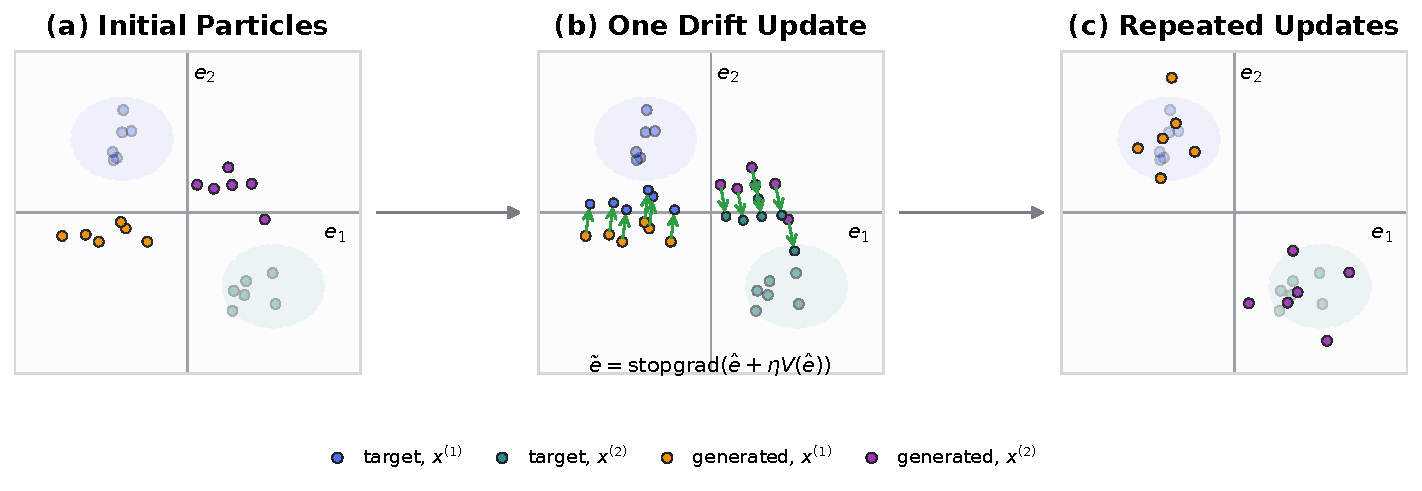
\includegraphics[width=0.62\textwidth]{figures/drifting_conditional_toy_figure_mpl.pdf}
\caption{Toy conditional particle simulation in residual space. Two inputs induce different target residual distributions. Starting from mismatched generated particles, the middle panel applies one attraction--repulsion drift update, and the last panel shows the particles after repeated updates.}
\label{fig:toy}
\end{figure*}

\begin{figure*}[t]
\centering
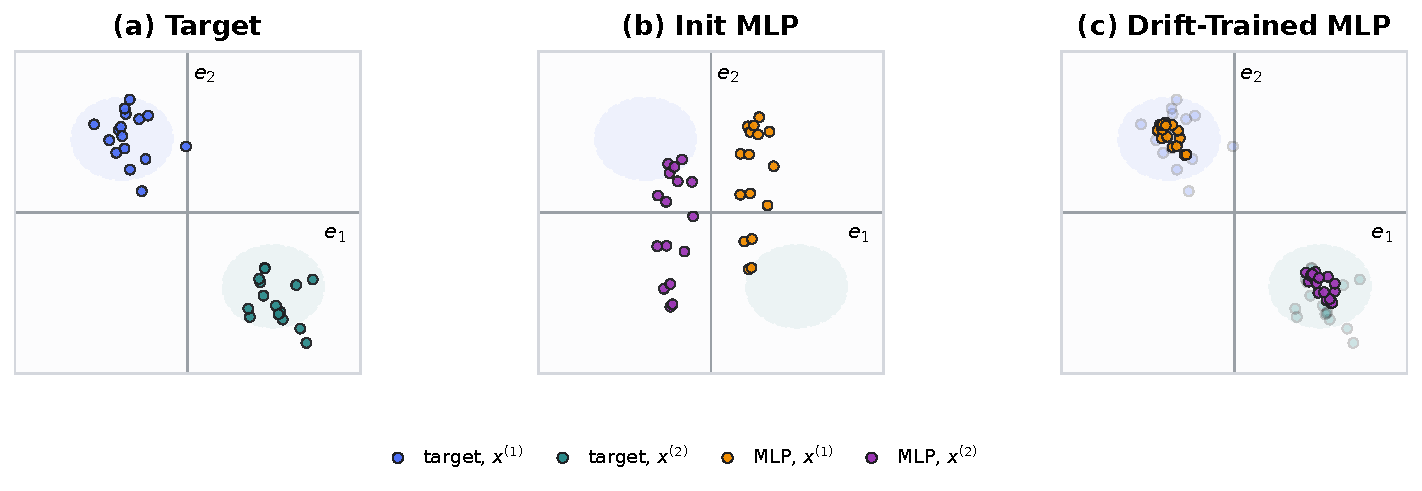
\includegraphics[width=0.62\textwidth]{figures/drifting_tiny_mlp_demo_mpl.pdf}
\caption{Toy conditional MLP trained with the drifting objective. The panels show target conditional residual samples, the randomly initialized generator, and the same generator after drifting training.}
\label{fig:toymlp}
\end{figure*}


\subsection{Conditional Channel Simulation}
We now specialize the generic drifting view to learned conditional channel simulation.
Let \(x \in \mathbb{R}^n\) denote the transmitted channel input and \(y \in \mathbb{R}^n\) the channel output.
The objective is to learn a conditional generator that reproduces the channel law given \(x\).
In this setting, conditioning enters through the transmitted symbol, while stochasticity is carried by a latent variable \(z \sim \mathcal{N}(0, I)\).

Two target parameterizations are useful in the experiments.
The first is the direct channel-output formulation, in which the generator approximates \(p(y | x)\) and predicts \(\hat{y} = g_\theta(x, z)\).
The second is the residual formulation, in which \(e = y - x\)
is modeled instead, so that the generator approximates \(p(e | x)\) and the channel output is reconstructed as \(\hat{y} = x + \hat{e}.\)
The direct formulation corresponds to learning the channel law itself, whereas the residual formulation injects the inductive bias that the channel output can be understood as the transmitted symbol plus a structured perturbation.
As discussed later in the experiments, the direct formulation aligns naturally with direct-output diffusion and WGAN baselines, while the residual formulation is often easier to optimize but can fall short on nonlinear channels.

%\begin{table}[t]
%$\caption{\textbf{Two target parameterizations for conditional drifting}}
%\label{tab:drifting_modes}
%\centering
%\tablestyle{5pt}{1.03}
%\tablefontsize
%%\begin{tabular}{@{}p{1.0cm}p{2.00cm}p{1.60cm}p{2.00cm}@{}}
%\toprule
%Mode & Output of \(g_\theta\) & Target object & Short interpretation \\
%\midrule
%Direct & \(\hat y\) & Learn \(p(y | x)\) & Learns the channel law %directly\\
%Residual & \(\hat e\), then \(\hat y=x+\hat e\) & Learn \(p(e | x)\) with \(e=y-x\) & Learns the channel perturbation\\
%\bottomrule
%\end{tabular}
%\end{table}

\subsection{Conditional Drifting Model}
  We use a practical conditional adaptation inspired by \cite{drifting}.
  To avoid confusion with the communication input symbol \(x\), we use \(u\) above for the generic
  sample variable in the abstract formulation and reserve \(x\) below for the transmitted symbol.
  In our implementation, drifting can be applied either in the direct-output space or in the residual space.
  In the direct mode, the generator predicts \(\hat y = g_\theta(x,z)\); in the residual mode, it predicts
  \(\hat e = g_\theta(x,z)\) with reconstruction \(\hat y = x + \hat e\), where \(z \sim \mathcal{N}(0, I).\)
  In both cases, \(g_\theta\) is implemented as a two-hidden-layer multilayer perceptron with hidden
  width \(128\), latent dimension \(16\), and SiLU activations:
\begin{equation}
[x, z]
\rightarrow
\mathrm{Linear}
\rightarrow
\mathrm{SiLU}
\rightarrow
\mathrm{Linear}
\rightarrow
\mathrm{SiLU}
\rightarrow
\mathrm{Linear}.
\end{equation}
The training target is formed from an attraction--repulsion drift field in the chosen target space. This is a concrete channel-specific instantiation of the generic field \(V_{p,q}\).
Given generated samples \(G = \{g_i\}\) and positive samples \(P = \{p_j\}\), we compute
\begin{equation}
V(g_i)
=
\left(
\sum_j w^{(P)}_{ij} p_j - g_i
\right)
-
\lambda
\left(
\sum_k w^{(G)}_{ik} g_k - g_i
\right),
\end{equation}
where \(w^{(P)}\) and \(w^{(G)}\) are row-normalized RBF kernel weights.
The first term attracts each generated sample toward a local barycenter of true samples in the chosen target space, and the second term repels it from nearby generated samples to reduce collapse.
This yields a detached target
\begin{equation}
\tilde{g}_i
=
\mathrm{stopgrad}\!\left(g_i + \eta V(g_i)\right),
\end{equation}
and the generator is optimized by
\begin{equation}
\mathcal{L}_{\text{drift}}
=
\frac{1}{|G|}
\sum_i
\left\|
g_i - \tilde{g}_i
\right\|_2^2.
\end{equation}
The generic update \(u \mapsto u + \eta V_{p,q}(u)\) is implemented as a kernel-based drift field estimated from minibatches of true and generated samples. The attraction term pulls generated samples toward the target cloud, and the repulsion term reduces collapse. This makes the update close in spirit to kernel-based distribution shaping and MMD-like matching, although we use it as a practical training rule rather than as a formal discrepancy-minimization objective.

In the simulations, the drift scale is \(\eta=1.0\), the repulsive weight is \(\lambda=1.0\), the minimum kernel bandwidth is \(0.2\), and the maximum drift norm is \(2.0\).
These settings are used throughout the drifting benchmark.

The major operational advantage is straightforward:
Once training is complete, sampling requires only a single evaluation of \(g_\theta(x,z)\).
In residual mode, this produces a channel residual sample \(\hat e\) followed by reconstruction \(\hat y=x+\hat e\). In direct mode, it produces \(\hat y\) directly.
There is no reverse chain, no ODE solver, and no per-sample iterative schedule at inference.

\paragraph{Conditioning-aware kernel variant.}
For the enhanced direct-output drifting model, we replace the target-only kernel by a condition-aware product kernel
  \[
  k\big((x_i,y_i),(x_j,y_j)\big)=k_x(x_i,x_j)\,k_y(y_i,y_j),
  \]
so that attraction and repulsion depend on similarity in both the channel input and the output space. In the direct-output setting, the target kernel can also incorporate residual similarity, yielding a drift field that is more closely aligned with the conditional channel structure. The generator architecture is unchanged.
With Gaussian factors, this is an RBF kernel on a scaled joint condition--output representation. It suppresses interactions between dissimilar transmitted symbols even when their outputs are close, so the drift uses conditionally relevant neighbors. The condition and target scales are \(0.5\) and \(1.0\), respectively.

%\begin{figure*}[t]
%\centering
%\input{figures/drifttrain_tikz.tex}
%\caption{Training-time drifting update for conditional channel residual modeling. For a fixed transmitted symbol \(x\), the generator produces residual samples \(\hat e_i\), which are moved toward the true residual cloud through a drift field that combines attraction to data and repulsion among generated samples. The network is then regressed toward the drifted targets.}
%\label{fig:drifttrain}
%\end{figure*}

%\begin{figure*}[t]
%\centering
%\input{figures/schematic_tikz.tex}
%\caption{Inference-time schematic for residual-mode conditional drifting. Once the generator has been trained, sampling requires only a single forward pass of \(g_\theta(x,z)\), followed by residual-to-output reconstruction. In the direct-output parameterization, the same one-shot generator would produce \(\hat y\) directly instead of \(\hat e\).}
%\label{fig:schematic}
%\end{figure*}



%\begin{figure*}[t]
%\centering
%\includegraphics[width=0.7\textwidth]{figures/toy_diffusion_oracle_demo_mpl.pdf}
%\caption{Oracle toy conditional diffusion trajectory on the same Gaussian conditional target. The panels show reverse-time snapshots from a 100-step diffusion process at \(t=100\), \(t=50\), \(t=20\), and \(t=0\). Starting from condition-independent noise, the reverse denoising trajectory progressively separates the conditions and contracts toward their target residual distributions. This figure is included to contrast the explicit multi-step reverse path of diffusion with the one-shot sampling path of drifting.}
%\label{fig:toydiff}
%\end{figure*}

\section{Experimental Setup}
\subsection{Channel Models}
We simulate four channel families. All channels are implemented on real-valued vectors.
For AWGN and Rayleigh, we use real-valued channel inputs and output vectors of length \(7\).
For SSPA and OptFib, the real-valued signal is interpreted in paired I/Q coordinates, with dimensions \(8\) and \(2\), respectively.
Noise is independent across real components unless the channel induces coupling.

\textbf{AWGN:}
\begin{equation}
y = x + n,
\qquad
n \sim \mathcal{N}(0,\sigma^2 I).
\end{equation}
This is the standard additive white Gaussian noise reference channel, serving as the simplest near-identity baseline.

\textbf{Rayleigh:}
The transmitted symbol is multiplied elementwise by a random fading amplitude and then corrupted by additive Gaussian noise:
\begin{equation}
y = h \odot x + n,
\end{equation}
where \(\odot\) denotes elementwise multiplication,
\begin{equation}
h_k = \frac{1}{\sqrt{2}}\sqrt{u_k^2 + v_k^2},
\qquad
u_k,v_k \overset{\text{i.i.d.}}{\sim} \mathcal{N}(0,1),
\end{equation}
and $n \sim \mathcal{N}(0,\sigma^2 I).$

Each real component is therefore scaled by an independent Rayleigh-distributed magnitude before noise is added.
This channel is multiplicative rather than additive and is correspondingly less aligned with a pure residual perturbation view.
%As implemented here, Rayleigh is also a real-valued vector channel rather than a paired-I/Q complex channel.
The fading amplitudes are latent and are not supplied as conditioning variables.

\textbf{SSPA:}
The input is passed through a smooth, solid-state power amplifier nonlinearity before additive noise is applied.
In this case, the real-valued representation is interpreted as paired I/Q components.
Let
\begin{equation}
r = \sqrt{x_I^2 + x_Q^2}
\end{equation}
denote the input amplitude.
The amplitude-dependent gain used in the benchmark is
\begin{equation}
a(r)
=
\frac{G}{\left(1+\left(\frac{Gr}{A_0}\right)^{2p}\right)^{1/(2p)}},
\end{equation}
with default parameters \(p=3\), \(A_0=1.5\), and \(G=5.0\).
The noiseless output is \(\tilde{x}=a(r)x\), with amplitude \(a(r)r\), and the observed channel output is
\begin{equation}
y = \tilde{x} + n,
\qquad
n \sim \mathcal{N}\!\left(0,\frac{\sigma^2}{2}I\right).
\end{equation}
This channel introduces amplitude-dependent nonlinear distortion while preserving the input direction in the I/Q plane.

%\textbf{OptFib:}
%We include a simplified memoryless optical-fiber proxy channel following \cite{li2018e2efiber} for the choice of parameters.
%As in SSPA, the real-valued state is interpreted as an I/Q pair.
%Let the state after propagation step \(k\) be \(x^{(k)} = [x_I^{(k)},x_Q^{(k)}]^\top\).
%At each step, the instantaneous nonlinear phase is
%\begin{equation}
%\phi^{(k)}
%=
%\gamma
%\left(\left(x_I^{(k)}\right)^2 + \left(x_Q^{(k)}\right)^2\right)\frac{L}%{K_{\text{step}}}.
%\end{equation}
%The deterministic Kerr-style rotation is
%\begin{equation}
%\begin{aligned}
%\tilde{x}_I^{(k+1)} &= x_I^{(k)}\cos\phi^{(k)} - x_Q^{(k)}\sin\phi^{(k)}, \\
%\tilde{x}_Q^{(k+1)} &= x_I^{(k)}\sin\phi^{(k)} + x_Q^{(k)}\cos\phi^{(k)},
%\end{aligned}
%\end{equation}
%followed by additive Gaussian perturbations at every step:
%\begin{equation}
%\begin{aligned}
%x_I^{(k+1)} &= \tilde{x}_I^{(k+1)} + \sigma_n \xi_I^{(k)}, \\
%x_Q^{(k+1)} &= \tilde{x}_Q^{(k+1)} + \sigma_n \xi_Q^{(k)},
%\end{aligned}
%\qquad
%\xi_I^{(k)},\xi_Q^{(k)} \overset{\text{i.i.d.}}{\sim} \mathcal{N}(0,1).
%\end{equation}
%When that optical-channel parameterization is used,
%\begin{equation}
%\sigma_n
%=
%\sqrt{\frac{10^{(P_n-30)/10}}{2K_{\text{step}}}},
%\end{equation}
%with \(P_n\) measured in dBm.

\textbf{OptFib:}
We include a simplified memoryless optical-fiber proxy channel following \cite{li2018e2efiber}. As in SSPA, the real-valued state is interpreted as an I/Q pair. Over \(K_{\text{step}}\) propagation steps, the state undergoes an amplitude-dependent Kerr-style phase rotation followed by additive Gaussian perturbation at each step. Writing \(x^{(k)}=[x_I^{(k)},x_Q^{(k)}]^\top\), the nonlinear phase is
\begin{equation}
\phi^{(k)}
=
\gamma \left(\left(x_I^{(k)}\right)^2 + \left(x_Q^{(k)}\right)^2\right)\frac{L}{K_{\text{step}}},
\end{equation}
and the next state is obtained by rotating \(x^{(k)}\) by \(\phi^{(k)}\) in the I/Q plane and adding Gaussian noise with per-step standard deviation
\begin{equation}
  \sigma_n
  =
  \sqrt{\frac{10^{(P_n-30)/10}}{2K_{\text{step}}}}.
\end{equation}



\subsection{Training Protocol}
This benchmark protocol closely follows the setup in \cite{kimicc2024}.
\paragraph{Channel settings}
For AWGN and Rayleigh, the setting is \(n=7\), while for SSPA it is \(n=8\). The corresponding \((E_b/N_0, R)\) pairs are \((5\,\mathrm{dB}, 4/7)\) for AWGN, \((12\,\mathrm{dB}, 4/7)\) for Rayleigh, and \((8\,\mathrm{dB}, 6/8)\) for SSPA, yielding noise standard deviations \(0.5260\), \(0.2350\), and \(0.3251\), respectively. For OptFib, the channel parameters are \(L=5000\), \(\gamma=1.27\), \(K_{\text{step}}=50\), and \(P_n=-21.3\) dBm.

\paragraph{Data and optimization settings}
For AWGN and Rayleigh, we use training dataset size \(10^7\), batch size \(5000\), and \(30\) epochs for drifting, diffusion, and WGAN. For SSPA, we use a training dataset size \(10^7\), batch size \(4096\), and \(160\) epochs for all three method families. For these three channels, we evaluate each method on \(10^6\) samples and use \(128\) sliced
Wasserstein distance (SWD) projections. OptFib is benchmarked separately with training dataset size \(120{,}000\), batch size \(512\), \(60\) training epochs, evaluation size \(100{,}000\), and \(256\) SWD projections.

\paragraph{Model settings}
Drifting uses a conditional MLP with latent dimension \(16\), hidden width \(128\), two hidden layers, \texttt{SiLU} activations, and Adam with learning rate \(10^{-3}\). The drifting objective uses drift scale \(1.0\), median-heuristic bandwidth selection, minimum bandwidth \(0.2\), maximum drift norm \(2.0\), and repulsive weight \(1.0\). We train both parameterizations: direct drifting with target \(y\) and residual drifting with target \(e=y-x\).

For AWGN, Rayleigh, and SSPA, diffusion models \(p(y | x)\) directly with \(v\)-prediction, cosine-ZF variance schedule, \(100\) diffusion steps, and EMA decay \(0.9\). Hidden widths are \(110\), \(128\), and \(110\), respectively. AWGN and Rayleigh use a two-stage learning-rate schedule (\(10\) epochs at \(10^{-3}\), then \(20\) epochs at \(10^{-4}\)), while SSPA uses a constant \(10^{-4}\) for \(160\) epochs. We report DDPM and DDIM with \(100\), \(50\), \(20\), and \(10\) denoising steps. For OptFib, diffusion uses residual modeling with \(\epsilon\)-prediction, standard cosine schedule, \(100\) steps, hidden width \(128\), learning rate \(10^{-3}\), and EMA decay \(0.995\).

WGAN uses a conditional Wasserstein objective with RMSprop at \(10^{-4}\) for generator and critic, five critic updates per generator update, and weight clipping at \(0.01\). Hidden widths are \(128\) (AWGN) and \(256\) (Rayleigh/SSPA). OptFib uses width \(128\).

\paragraph{Experimental Fairness} The benchmark is intended as a practical comparative study rather than a strict matched-capacity comparison. The inference networks have the same order of magnitude but are not exactly matched: drifting uses about \(19\)--\(21\)k generator parameters, diffusion uses \(60\)--\(74\)k denoiser parameters, and WGAN uses \(17\)--\(72\)k generator parameters depending on the channel. DDPM and DDIM share denoiser weights. Training schedules were chosen as stable implementations for each model family. A stricter matched-capacity study is left for future work.
Table~\ref{tab:benchmark-all-channels} reports the mean and standard deviation over ten independent training seeds, using the same seed indices across methods within each channel.
%To compare distributional accuracy and latency with the model capacity, Table~\ref{tab:model-size} reports inference-network parameter counts used in this benchmark.

%\input{model_size_table.tex}
%\paragraph{Seeding and reporting.}
%  All benchmark results are reported as mean \(\pm\) standard deviation over ten seeds.
%  Each run uses deterministic initialization to reduce run-to-run variance unrelated to model
%  stochasticity.


\subsection{Evaluation Metric}
We focus on generator-level distributional accuracy and timing rather than full end-to-end communication metrics such as SER or \(E_b/N_0\) curves, to reduce encoder--decoder dependency in the comparison.
The primary metric is SWD, computed in the target space used by each benchmark path.
For direct-output models, we report \(\mathrm{SWD}\!\left(\{\hat{y}_i\}, \{y_i\}\right)\). For residual models, we report \(\mathrm{SWD}\!\left(\{\hat{e}_i\}, \{e_i\}\right)\).
Given true samples \(P=\{v_i\}_{i=1}^N\) and generated samples \(Q=\{\hat v_i\}_{i=1}^N\), SWD is estimated by drawing random unit directions \(\theta_m\), projecting both clouds onto those directions, computing the one-dimensional Wasserstein distance for each projection, and averaging over projections:
\begin{equation*}
\mathrm{SWD}(P,Q)
=
\frac{1}{M}
\sum_{m=1}^M
W_1\!\left(\{\langle \theta_m,v_i\rangle\}_{i=1}^N,\{\langle \theta_m,\hat v_i\rangle\}_{i=1}^N\right).
\end{equation*}
Thus, SWD compares the generated and true sample clouds through many one-dimensional views and captures geometric mismatch more faithfully than a purely bin-based marginal comparison. In our experiments, SWD is estimated using \(128\) random one-dimensional projections on AWGN,
  Rayleigh, SSPA, and \(256\) projections on the separate OptFib benchmark.
SWD is used primarily for comparability with prior diffusion-channel benchmarks \cite{paper2309,kimicc2024}. Compared with histogram-based \(L_1\) distance, it also better captures sample geometry in \(\mathbb{R}^n\). While SWD provides a geometry-aware comparison of conditional output distributions, it does not directly capture decision-relevant behavior such as error rates, which depend on the joint structure of $(x,y)$.


\section{Results}
\subsection{Main SWD Benchmark Across Channels}
Table~\ref{tab:benchmark-all-channels} reports the SWD benchmark across AWGN, Rayleigh, SSPA, and
OptFib. Direct output-space SWD is used throughout the table except for the additional residual-
native row ``Drifting (res., \(e\))'', which reports residual-space SWD for the residual
parameterization. DDIM-100 achieves the lowest direct-space SWD on AWGN, Rayleigh, and SSPA, while
DDPM is strongest on OptFib. Among the one-shot generators under direct-space evaluation, direct-
output drifting is consistently strongest across all four channels, whereas residual drifting
degrades substantially once judged against the full \(p(y | x)\) relation. The additional
residual-space row makes clear that residual drifting remains strong in its native target space.
Reduced-step DDIM variants degrade systematically as the number of sampling steps is reduced. This indicates that residual drifting is best interpreted as a specialized residual-matching surrogate rather than a uniformly strong full output-space channel model.

Timing results follow the expected pattern: Drifting and WGAN operate at roughly \(0.38\) to
\(0.42\,\mu\mathrm{s}\) per sample, whereas DDPM and DDIM range from about \(0.01\) to \(0.13\,
\mathrm{ms}\), depending on the sampler and the number of denoising steps. Inference timings used
an NVIDIA GeForce RTX 5060 Ti and seven CUDA-synchronized repeats (batch size \(512\), \(40\)
batches; maximum relative standard deviation \(1.4\%\)). Thus, even when diffusion achieves the
strongest SWD, one-shot generators retain a substantial practical latency advantage.
\begin{table*}[t]
\centering
\caption{\textbf{Ten-seed SWD benchmark across all channels.} Lower is better. Direct output-space SWD is reported unless the row label explicitly indicates residual-space SWD. The residual-space row is included for diagnostic purposes only.}
\label{tab:benchmark-all-channels}
\tablestyle{6.5pt}{1.03}
\tablefontsize
\begin{tabular}{@{}lcccc@{}}
\toprule
Method & AWGN & Rayleigh & SSPA & OptFib \\
\midrule
\rowcolor[gray]{0.9} \multicolumn{5}{l}{\textit{One-shot generators}} \\
\headspace Drifting (dir.) & 0.0100 $\pm$ 0.0007 & 0.0085 $\pm$ 0.0012 & \textbf{0.0060} $\pm$ 0.0008 & \textbf{0.0275} $\pm$ 0.0104 \\
\headspace Drifting (res., $y$) & 0.0670 $\pm$ 0.0138 & 0.3681 $\pm$ 0.0031 & 0.4812 $\pm$ 0.0022 & 0.3864 $\pm$ 0.0211 \\
\headspace Drifting (res., $e$)[residual space] & \textbf{0.0097} $\pm$ 0.0009 & \textbf{0.0062} $\pm$ 0.0009 & 0.0130 $\pm$ 0.0003 & 0.0463 $\pm$ 0.0082 \\
\headspace Paper WGAN & 0.0198 $\pm$ 0.0050 & 0.0171 $\pm$ 0.0050 & 0.0287 $\pm$ 0.0156 & 0.0414 $\pm$ 0.0179 \\
\midrule
\rowcolor[gray]{0.9} \multicolumn{5}{l}{\textit{Diffusion samplers}} \\
\headspace DDPM & 0.0070 $\pm$ 0.0004 & 0.0079 $\pm$ 0.0008 & 0.0032 $\pm$ 0.0005 & \textbf{0.0088} $\pm$ 0.0019 \\
\headspace DDIM-100 & \textbf{0.0042} $\pm$ 0.0006 & \textbf{0.0044} $\pm$ 0.0007 & \textbf{0.0024} $\pm$ 0.0004 & 0.0584 $\pm$ 0.0148 \\
\headspace DDIM-50 & 0.0064 $\pm$ 0.0004 & 0.0066 $\pm$ 0.0010 & 0.0030 $\pm$ 0.0005 & -- \\
\headspace DDIM-20 & 0.0143 $\pm$ 0.0003 & 0.0146 $\pm$ 0.0014 & 0.0056 $\pm$ 0.0006 & -- \\
\headspace DDIM-10 & 0.0264 $\pm$ 0.0004 & 0.0271 $\pm$ 0.0013 & 0.0092 $\pm$ 0.0008 & -- \\
\bottomrule
\end{tabular}
\end{table*}



Figure~\ref{fig:awgn-ser-symbolic} reports symbolic AWGN SER for a \((4,7)\) autoencoder trained through analytic and learned channel surrogates. Diffusion and WGAN remain closest to the analytic-channel baseline. In the seed-7 experiment, the conditioning-aware kernel reduces direct-drifting SER from \(1.60\times10^{-2}\) to \(7.55\times10^{-3}\) at \(5\,\mathrm{dB}\), and from \(3.50\times10^{-4}\) to \(7.00\times10^{-5}\) at \(8\,\mathrm{dB}\). It improves upon standard direct drifting while also showing that generator-level SWD does not map one-to-one to downstream performance.


\begin{figure}[t]
\centering
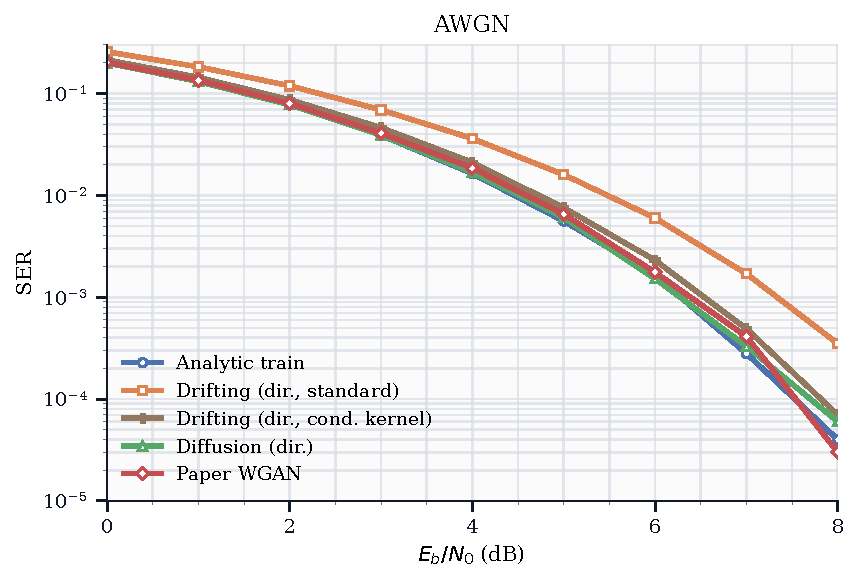
\includegraphics[width=0.95\columnwidth]{awgn_ser_symbolic_direct_compare.pdf}
\caption{End-to-end symbolic AWGN SER for a \((4,7)\) autoencoder trained through analytic and learned channel surrogates. Diffusion and WGAN remain closest to the analytic baseline, while the conditioning-aware direct drifting variant improves upon standard direct drifting. This illustrates that generator-level metrics such as SWD do not fully capture decision-relevant structure.}
\label{fig:awgn-ser-symbolic}
\vspace{-1em}
\end{figure}

\smallskip
\noindent\textit{Remark on metric limitations.}
SWD measures output-distribution geometry independently of a particular receiver, whereas SER tests whether the learned conditional law preserves the decision-relevant structure used by one encoder--decoder pair. The two measurements are complementary, and neither alone gives a complete assessment.


%\input{partial_direct_metric_table.tex}
\section{Conclusion}
This paper studied conditional drifting models for learned channel simulation and compared them with conditional diffusion and WGAN baselines on AWGN, Rayleigh, SSPA, and optical-fiber proxy channels. The results show a clear tradeoff between fidelity and latency. Diffusion provides the strongest distributional accuracy overall, while drifting remains competitive and retains the one-shot advantage with substantially lower inference cost. 
Under direct output-space evaluation, direct-output drifting is the strongest one-shot generator across the main benchmark. The additional residual-space row shows that residual drifting remains strong when evaluated in its native residual target space, but that this advantage does not transfer to full output-space matching. These results suggest that drifting is a practically relevant direction for learned channel simulation, especially when low-latency generation matters. More broadly, these experiments highlight the importance of understanding how generator-level SWD relates to downstream communication performance and motivate further study of channel-specific kernel design for improving direct-output drifting.
Future work should extend the comparison to broader channel families, including MIMO, memory, and more realistic optical channels, together with downstream communication metrics. A more formal analysis of the drift objective and its kernel dependence is left for future work.
\bibliographystyle{IEEEtran}
\bibliography{references}

\end{document}
